%----------------------------------------------------------------------------------------
%	PACKAGES AND DOCUMENT CONFIGURATIONS
%----------------------------------------------------------------------------------------

\documentclass[10pt,a4paper]{article}
%\DeclareUnicodeCharacter{0301}{*************************************}

% Adjusting margins to personal my need
\addtolength{\oddsidemargin}{-.5in}
\addtolength{\evensidemargin}{-.5in}
\addtolength{\textwidth}{1in}
\addtolength{\topmargin}{-.5in}
\addtolength{\textheight}{1in}

% Graphics
\usepackage{caption}
\usepackage{subcaption}
\usepackage{graphicx}
\graphicspath{{figures/}}
\usepackage{float}

% Math
\usepackage{amssymb}
\usepackage{amsmath} % Required for some math elements 
\usepackage{numprint}

% Other
\usepackage{algorithmic}
\usepackage{array}
\usepackage{lipsum}
\usepackage{hyperref}

%Bibliography
\usepackage[citestyle=numeric-comp,bibstyle=numeric-comp,autopunct=true,sorting=none,bibencoding=utf8]{biblatex}
\bibliography{bibliography/sources}

%indent the first paragraph as well
%\usepackage{indentfirst}
\setlength{\parindent}{0em}

% code highlighting
\usepackage{listings}
\usepackage{color}

\definecolor{mygreen}{rgb}{0,0.6,0}
\definecolor{mygray}{rgb}{0.5,0.5,0.5}
\definecolor{mymauve}{rgb}{0.58,0,0.82}

\lstset{ %
  backgroundcolor=\color{white},   % choose the background color
  basicstyle=\footnotesize,        % size of fonts used for the code
  breaklines=true,                 % automatic line breaking only at whitespace
  captionpos=b,                    % sets the caption-position to bottom
  commentstyle=\color{mygreen},    % comment style
  escapeinside={\%*}{*)},          % if you want to add LaTeX within your code
  keywordstyle=\color{blue},       % keyword style
  stringstyle=\color{mymauve},     % string literal style
}
{}

% caption
\usepackage{caption}
\captionsetup[table]{font={small,stretch=0.5}, skip=5pt, position=above, labelfont=bf}
\captionsetup[figure]{labelfont=bf}
\usepackage{booktabs}
\usepackage{siunitx}  
\sisetup{
    table-format = -1.3e-1,
    table-number-alignment = center,
    table-auto-round
  }
%\usepackage{longtable}

%----------------------------------------------------------------------------------------
%	MAIN PART
%----------------------------------------------------------------------------------------
\begin{document}

\title{Appliance of SAveRUNNER to identify repurposable drugs for treatment of COVID-19}% Title
\author{Sean Klein \\1992143}
% \date{\today} % Date for the report
\maketitle % Inserts the title, author and date

%----------------------------------------------------------------------------------------
%	Abstract
%----------------------------------------------------------------------------------------
\begin{abstract}
\normalsize
The worldwide outbreak of severe acute respiratory syndrome coronavirus 2 and associated coronavirus disease 2019 requires not only effective vaccines for prevention but also medication for the treatment of already infected. It is important that these drugs are available for widespread usage as soon as possible. Drug repurposing is an approach that accelerates the time and reduces the cost of drug development by the investigation of drugs approved by the Food and Drug Administration (FDA) for other diseases already. We use SAveRUNNER to perform network analysis to find drugs that have the potential to be repurposed.

\end{abstract}
\thispagestyle{empty}
\clearpage

%----------------------------------------------------------------------------------------
%	Table of Content
%----------------------------------------------------------------------------------------
\setcounter{tocdepth}{2}
%\tableofcontents
%\clearpage

%----------------------------------------------------------------------------------------
%	Main Part
%----------------------------------------------------------------------------------------
\section{Introduction}

%\lipsum[8]

%\lipsum[8]

% scientific Issue

% state of the art -> scientific literature results
% new Hypothesis and required knowledge
% overview of contents of following sections
% clearly state the aims of the study
% relevance of the results

% SAveRUNNER Hypothesis
% drug targets and associated disease genes/modules are nearby in the interactome map
% looking for high similarity values
% the program quantifies interplay between drug targets and disease proteins (# of edges) 

The Coronavirus disease 2019 (COVID-19) pandemic is the third outbreak of coronavirus-related disease of the 21st century. What all three have in common is the unpredicted emergence, rapid and easy proliferation that leads to harsh consequences in each case. However, they do differ in the characteristics of the diseases.\\
The first outbreak, Severe acute respiratory syndrome (SARS), was caused by severe acute respiratory syndrome coronavirus (SARS-CoV-1). The SARS disease first occurred in Foshan, China in November 2002. In 2003 the infections happened globally, leading to a ~10\% fatality rate.
The disease caused by Middle East respiratory syndrome coronavirus (MERS-CoV) first emerged at Jeddah in Saudi Arabia in 2012 and developed a fatality rate of ~35\% globally \cite{Kirtipal_2020}. 
COVID-19, which is caused by SARS-CoV-2, has a much lower fatality rate which is below 3\% in most countries \cite{Mathieu2021, Yi_2020}. It is important to note that the former two outbreaks have much lower counted infections than COVID-19. In summary, COVID-19 spreads much faster and more successful, but leads to fewer deaths among the infected. This makes the disease harder to control and allowed the outbreak to reach a scale and severity not known before from Covid-19's predecessors. 
In addition, there appears to be a similarity in symptoms as well. The main early symptoms, fever, dry cough, dyspnea, and diarrhea occurred in similar percentages among the infected for all three diseases. However, MERS patients required ventilation support in 80\%  of cases. For SARS and COVID-19, this number is less than 20\% and only 8\% respectively \cite{Yi_2020}.
Further symptoms of COVID-19 include shortness of breath, muscle ache, dizziness, headache, sore throat, rhinorrhea, chest pain, diarrhea, nausea, vomiting, hypoxemia, acute respiratory syndrome, septic shock, metabolic acidosis, and coagulopathy. 
Furthermore, atypical pneumonia, acute lung injury, and acute respiratory distress syndrome (ARDS) are associated with the worst chest radiographic findings in patients \cite{Yi_2020}.
In addition, all three viruses are believed to originate from bats, which are believed to be hosts of emerging viral pathogens due to their unique immune systems, their densely packed colonies, longevity, and ability to fly which allows spread at a fast rate. Bats act as host to other coronaviruses as well \cite{Kirtipal_2020}.
The intermediate hosts for SARS, MERS, and COVID-19 are believed to be civet cats, camels, and pangolins respectively. The latter is based on a 99\% similarity of SARS-CoV-2 and another coronavirus found in the pangolin \cite{Yi_2020}. This information is crucial for cutting the transmission line to prevent re-emergence in the future. 
Infection takes place via person‐to‐person interactions, transmission by aerosols, and transmission by touch. The transmission is also influenced by several environmental factors. For instance, when the temperature is high, the rate of transmission is inhibited. impact of maximum air humidity and wind speed on the prevalence of COVID‐19 has been found not to be statistically significant \cite{Sreekanth_Reddy_2020}. \\

The virus body of SARS-CoV-2 consists of a single-stranded RNA genome and a protein hull surrounding it. The viral spike glycoprotein of SARS-CoV-2 was found to interact with Angiotensin-converting enzyme 2 (ACE2) on the cells membrane to trigger membrane fusion of the virus and its host. Thus all cells that express ACE2 (lung, kidney \& gastrointestinal system) are targets of SARS-CoV-2. Despite that respiratory failure remains the primary cause of death \cite{Yi_2020}.
Without going into too much detail about the human immune response, it is important to note that later stages of COVID-19 are characterized by a cytokine storm causing hyper-inflammation. Furthermore, SARS-CoV-2 possesses the ability to halt T cell function and to induce their apoptosis as well as causing pyroptosis in lymphocytes and macrophages \cite{Kirtipal_2020}.
Overall, the genome of corona-viruses shows high flexibility in terms of gene content and recombination. In one investigation, the spike protein was found to have the most variation in
its active sites while other structural proteins (eg. the E protein) were highly conserved \cite{Ahmadi_2021}. This raises the question of whether other proteins are better suited for vaccines than the currently used spike protein. \\

There are two main groups of drugs that are currently considered for the treatment of COVID-19. Those are antiviral \& immunomodulatory drugs. There are other candidates as well, which cannot be grouped as easily \cite{Bartoli_2021}. Favipiravir (FPV) and Remdesivir (RDV) appear to be the most promising antiviral drugs but many more have been suggested \cite{Yi_2020, Mohamed_2021, Sreekanth_Reddy_2020}. PFV is a type of RNA-dependent RNA polymerase (RdRp) inhibitor. It is also known as T-705 and was being developed in 2002 as an inhibitor of influenza. It selectively inhibits the viral RNA-dependent RNA polymerase or causes lethal mutagenesis upon incorporation into the virus RNA without cytotoxicity to mammalian cells \cite{Ghasemnejad_Berenji_2020}. This repurposable drug has already been shown to be effective against other single-stranded RNA viruses as well \cite{Ghasemnejad_Berenji_2020, Sreekanth_Reddy_2020}. In addition, it already has been tested in clinical trials in China and has proven to be effective in reducing viral replication. However, the drug has many adverse side effects that make universal and widespread use in the future difficult. Still, these effects are significantly fewer than in some other candidates, such as lopinavir and ritonavir \cite{Ghasemnejad_Berenji_2020}.
Meanwhile, RDV appears to be the most effective antiviral drug proposed so far \cite{Bartoli_2021}. This drug also interacts with the RdRp leading to premature termination of viral RNA replication \cite{Sreekanth_Reddy_2020}. At least in one study, this drug showed no direct negative effects in the patient \cite{Holshue_2020}. It is also the first agent recommended for authorization in the European Union (EU) for use in the treatment of COIVID‐19 \cite{Sreekanth_Reddy_2020}.
Both, FPV and RDV, have also shown little drug-drug interaction with antipsychotic drugs, making them safer to use in the affected patient group \cite{Plasencia_Garc_a_2021}.
Immunomodulatory include corticosteroids like dexamethasone and other drugs, which might be useful in the inflammatory phase of the disease \cite{Bartoli_2021}. Other Inflammation inhibitors, such as anti-IL6, anti-IL1 and are valuable candidates for treatment in advanced stages as well \cite{Stasi_2020, Saeed_2021}.
Azithromycin is another interesting candidate as it combines antiviral and immunomodulatory properties. It has the ability to downregulate cytokine production, maintain epithelial integrity, and prevent lung fibrosis could play a role in the hyperinflammatory stage \cite{Echeverr_a_Esnal_2020}.
Among the other drugs that are suggested are antimalarials like chloroquine and hydroxychloroquine that could have a beneficial effect on COVID-19 through multiple molecular effects \cite{Ong_2020}. In addition to these conventional drugs, efforts on the use of plant-based and traditional Chinese medicine have been made as well, some showing positive results \cite{Yi_2020, Boozari_2020, Adhikari_2020}
\\

Here, we performed network analysis on the human interactome using SAveRUNNER to discover new potential candidates for drug repurposing \cite{Fiscon2020, Fiscon2021}. This process allows finding drugs that have already been approved by the FDA to be used in other diseases.
The benefit of repurposed drugs is less time and lower cost required until the drug can be administered commonly for treatment. As some of the approval steps don't have to be repeated or can be significantly shortened. Although a lot of research has been conducted already, it is still beneficial to cross-check pre-existing results and potentially reveal new candidates to be used for the treatment of COVID-19.


%%%%%%%%% Resterampe

%  10.1002/cbic.202000595 Sreekanth_Reddy_2020
% Coronavirus disease 2019 (COVID‐19) emerges as an infectious disease whose mortality rate is ill‐elucidated because of the difficulty in quantifying the number of asymptomatic and undiagnosed deaths. [1] While some COVID‐19 patients display mild symptoms, others die within a few days after infection.

% https://dx.doi.org/10.1007%2Fs00213-020-05716-4 Plasencia_Garc_a_2021
% The main interactions between COVID-19 drugs and antipsychotics are the risk of QT prolongation and/or TdP, and CYP interactions.
% COVID-19 drugs and antipsychotics are the risk of QT-prolongation and TdP, and cytochromes P450 interactions
% Remdesivir, baricinitib, and anakinra can be used concomitantly with antipsychotics without risk of drug-drug interaction (except for hematological risk with clozapine and baricinitib)
% Favipiravir only needs caution with chlorpromazine and quetiapine.
% Tocilizumab is rather safe to use in combination with antipsychotics. 
% The most demanding COVID-19 treatments for coadministration with antipsychotics are chloroquine, hydroxychloroquine, azithromycin, and lopinavir/ritonavir because of the risk of QT prolongation and TdP and cytochromes interactions

% 10.1007/s12035-020-02093-z Ong_2020
% COVID-19 is a pro-inflammatory-driven condition with loss of smell and taste, suggesting that it may affect the olfactory and gustatory systems and the brain. These effects may persist even after the virus has been cleared from the body

% 10.1016/j.ejphar.2020.173644 Stasi_2020
%  first stage: characterised by upper respiratory tract infection, accompanied by fever, muscle fatigue and pain. Nausea or vomiting and diarrhoea are infrequent in this initial stage of the disease
% second stage - onset of dyspnoea and pneumonia.
%  third stage - worsening clinical scenario dominated by a cytokine storm and the consequent hyperinflammatory state -> leading arterial and venous vasculopathy in the lung with thrombosis of the small vessels and evolution towards serious lung lesions up to ARDS etc.
% fourth stage -> death or recover
\clearpage

\section{Materials and Methods}
\label{sec:Methods}

\subsection{SAveRUNNER}

For the project, the most recent code (as of 08.12.21) found on the SAveRUNNER Github repository
%\footnote{\url{https://github.com/sportingCode/SAveRUNNER}} 
was used on the diseases "COVID-19" and "Severe Acute Respiratory Syndrome" \cite{Fiscon2021}.
The similarity metric was used for the edge-weights ("interaction"). The p-value threshold was set to 0.05 and the options \verb|adjust_link| and \verb|new_link| were set to \verb|T| and \verb|F| respectively.
Furthermore, a Subnetwork was computed for COVID-19 as well.
Any other variable of the program remained at their default values as well. 
The tool also produces some interesting figures automatically. Included here are figures \ref{fig:DieseaseDiesease} and \ref{fig:DrugDiesease}.
\subsection{Deriving original medical indications}

For deriving the original medical indication of the drugs proposed by SAveRUNNER, the therapeutic target database was used. The corresponding data and code were provided by Dr. Giulia Fiscon as well. All diseases that occurred more than once were visualized in a horizontal bar plot using python (version 3.7.12) and the package \verb|pandas| (version 1.1.5).

\subsection{Network Plot}

The Visualization of the computed network was created using Cytoscape 3.9.0 \cite{Shannon2003}. The "Edge-weighted Spring Embedded Layout" was used with the adjusted-similarity values. All Drug Labels were hidden. Edges were colored via continuous color-scale based on the adjusted similarities as well.


\clearpage

\section{Results and Discussion}
\label{sec:methodology}

% QC score rewards if drug and disease genes are placed in the same cluster, no penalty if not


% TODO
% disease-disease lists drugs with two common drugs per row: Drug - Disease of Interest - other Disease -> Visualize BIPARTITE GRAPH (not that relevant for me)

% find smth that could be related to target disease
% org med indication -> paper that relates drug to some mechanism
% -¨- -> look at most represented onLabel disease

% ==> try to find out if prediction could make sense

\subsection{Predicted repurposable drugs for COVID-19}

Table \ref{tab:predDrugsCovid} shows the first 20 drugs predicted by SAveRUNNER for COVID-19 sorted by the associated p-values in ascending order. In total 101 repurposable drugs were predicted for COVID-19.

\begin{table}[H]
\begin{center}
%\parbox{11cm}{
\captionsetup{width=10.5cm}
\caption{Predicted repurposable drugs for COVID-19. Values are sorted by p-values and are also rounded to three decimals. Only the drugs with 20 lowest p values are shown.}
\label{tab:predDrugsCovid}
%}
\npdecimalsign{.}
\begin{tabular}{ l S S }
    \toprule
    \text{Drug} & \text{p-Value} & \text{Adjusted Similarity} \\
    \midrule
azacitidine     & 1.698e-07 & 1.000e+00             \\
riboflavin      & 1.910e-06 & 9.932e-01             \\
noscapine       & 9.400e-06 & 1.000e+00             \\
phylloquinone   & 1.288e-05 & 9.994e-01             \\
flavin adenine dinucleotide & 4.693e-05 & 9.631e-01 \\
decitabine      & 9.737e-05 & 1.000e+00             \\
isoniazid       & 1.047e-04 & 9.932e-01             \\
tadalafil       & 1.064e-04 & 9.932e-01             \\
avanafil        & 1.373e-04 & 9.932e-01             \\
latanoprost     & 1.435e-04 & 9.932e-01             \\
telotristat ethyl & 4.260e-04 & 9.932e-01           \\
kappadione      & 5.929e-04 & 9.967e-01             \\
sapropterin     & 7.441e-04 & 9.932e-01             \\
ixekizumab      & 7.785e-04 & 9.932e-01             \\
menadione       & 8.224e-04 & 9.856e-01             \\
anisindione     & 1.231e-03 & 1.000e+00             \\
roflumilast     & 1.361e-03 & 9.932e-01             \\
papaverine      & 1.378e-03 & 9.932e-01             \\
acrivastine     & 1.418e-03 & 9.932e-01             \\
flucytosine     & 2.170e-03 & 1.000e+00             \\

\bottomrule
\end{tabular}
\npnoround

\end{center}
\end{table}

For the drug with the lowest p-value, Azacitidine, there is at least one reported case where this drug was involved in the successful treatment of COVID-19 \cite{Taurino_2021}. However, this patient also suffered from pneumonia and concurrent acute myeloid leukemia, which is one of the target diseases of Azacitidine \cite{Wishart2017}. It is questionable how much impact Azacitidine had in defense against SARS-CoV-2. Despite that, the results from SAveRUNNER makes this case worth investigating.\\
Next on table \ref{tab:predDrugsCovid} is Riboflavin, which is a vitamin to correct vitamin B2 deficiency \cite{Wishart2017}. Multiple publications report a positive effect of Riboflavin in combination with UV light regarding the concentration of SARS-CoV-2 in liquid samples (blood or plasma) \cite{Ragan_2020, Yonemura_2021}. \\
Noscapine, the drug with the 3rd lowest p-value, is used against the common cold, coughs and respiratory diseases \cite{Wishart2017}. These symptoms are some of the most common symptoms found in COVID-19 patients, hence it appears worth investigating whether the symptomatic treatment increases the recovery rate of patients. \\
Phylloquinone appears to be the generic name for Vitamin K1. Not much information is available on K1 in regards to COVID-19. However, two investigations note the connection to the so-called endothelial protein S which appears to be able to prevent the cytokine storm observed in COVID-19 cases \cite{Popa_2021, Dofferhoff_2020}. Furthermore, vitamin K depletion has been reported in COVID-19 patients \cite{Dofferhoff_2020}. This suggests that administration of this vitamin may allow to lessen the severity or prevent the cytokine storm. This over-reaction of the immune system occurs during the most severe stage of the disease. If it could be lessened, the already weakened patients may have higher chances of survival.


% --------------------------------------------------------------------------------

\subsection{Matched on-Label diseases of predicted drugs}

Figure \ref{fig:onLabel} shows the original (on-label) targets for the predicted drugs, according to the therapeutic drug database \cite{Zhou_2022}, which may be interesting for several reasons. For once, on-label and off-label diseases might share a certain characteristic, symptoms for example. This might then help to further explain the repurposability of a certain drug or group of drugs.
Furthermore, the proximity of the on-label and off-label disease modules in the underlying protein interactome can potentially be reflected in such an analysis as well.

\begin{figure}[H]
    \captionsetup{width=0.7\textwidth}
    \centering
    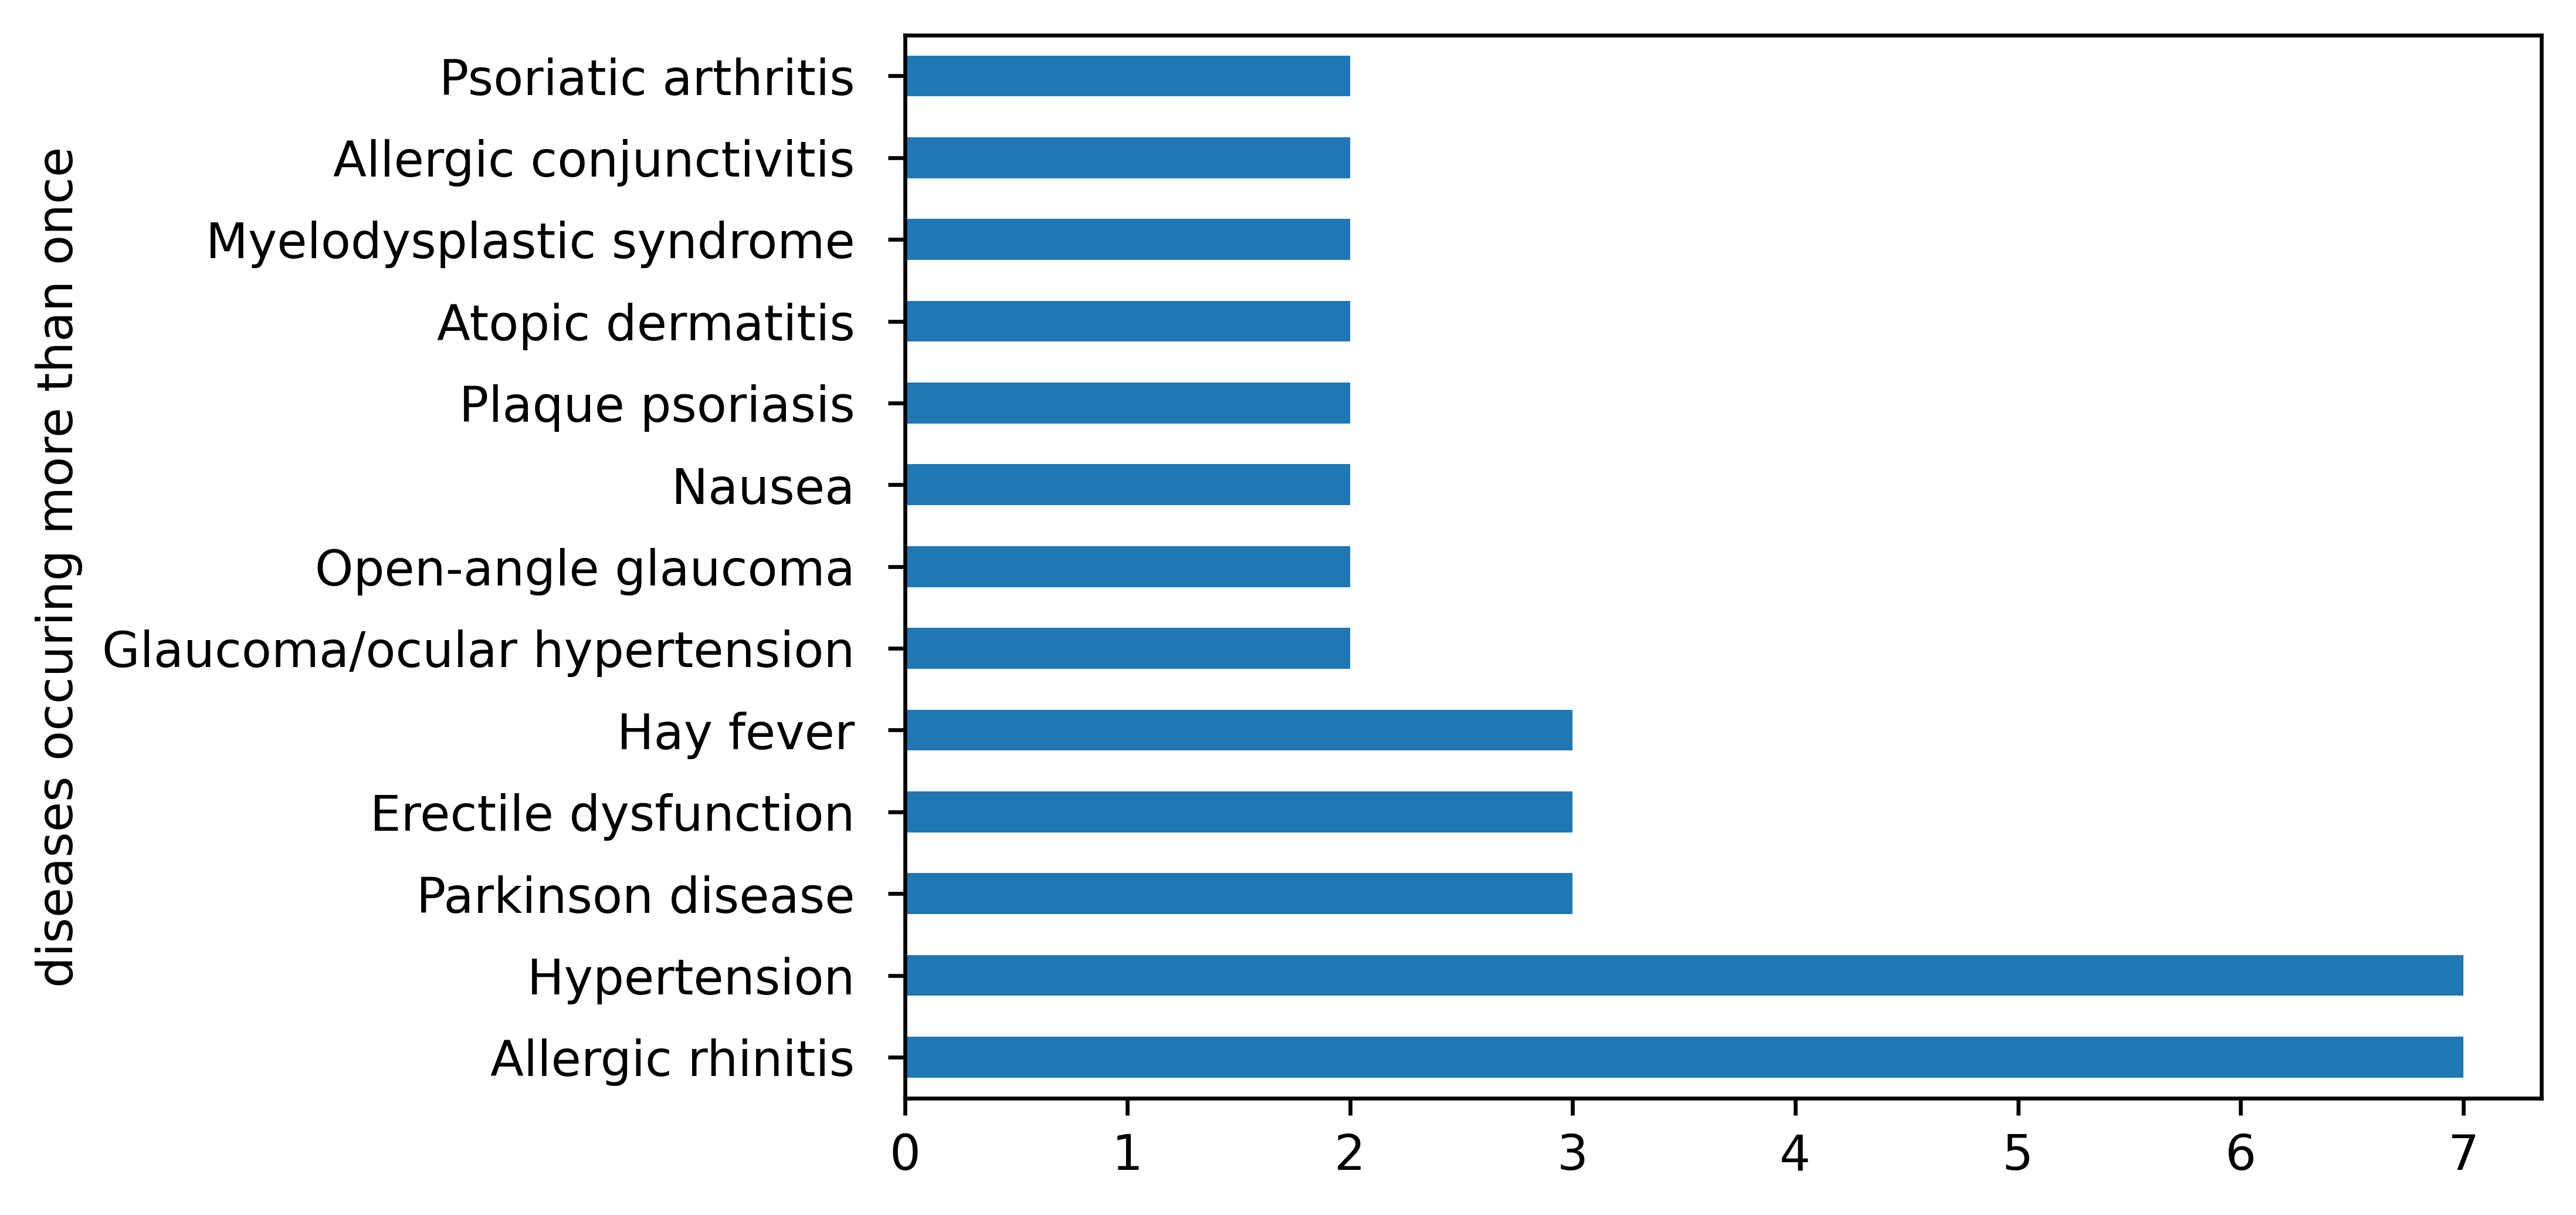
\includegraphics[width=0.7\textwidth]{figures/onLabel_diseases_saverunner_covid.png}
    \caption{On Label targets for drugs predicted by SAveRUNNER that occur more than once.}
    \label{fig:onLabel}
\end{figure}

Some of the hypertension-related drugs will be investigated in the next section. These three as well as deserpidine and Perindopril all affect the ACE protein, which is vital in the infection process of SARS-CoV-2. Another drug in this group, verapamil, does not affect ACE according to the DrugBank \cite{Wishart2017}. However, the adjusted similarity for this drug is also lower than for the ACE-inhibiting drugs. This drug is either not beneficial for the treatment of COVID-19 after all (but still close enough to the disease module in the interactome) or is potentially useful in another way. This would require further investigations.
The drugs associated with Allergic rhinitis are more difficult to link to COVID-19. Methdilazine, Clemastine, Cetirizine, and Fexofenadine all interact with H1 histamine receptor or act as antagonists to histamine $H_{1}$ \cite{Wishart2017}. As SARS-CoV-2 interacts with different parts of the immune system, these drugs' targets might be close enough in the network to lead to positive results by SAveRUNNER. Whether there is an actual molecular benefit for COVID-19 treatment needs to be investigated as well. Interestingly two publications investigating drugs related to histamine H2 receptor could not find any benefits for treatment of COVID-19 or suggested monitoring of patients during treatment with these drugs due to severe adverse effects \cite{Kim_2021, Chiu_2021}. Whether this translates to having similar effects for the H1 histamine receptor is uncertain.

% --------------------------------------------------------------------------------

\newpage
\subsection{Overlap with SARS}

Since SARS-CoV-2 has a genome sequence that is 75–80\% identical to that of SARS-CoV-1, it makes sense to look at drugs that could be used for both diseases \cite{Ghasemnejad_Berenji_2020}. Multi-target therapeutic agents have other benefits. Those can be better predictive pharmacokinetics, better patient compliance and reduced risk of drug interactions \cite{Mohamed_2021}.\\
Figure \ref{fig:Network} presents the Drug-Disease network for SARS and COVID-19. An edge is drawn between a drug (circular node) and a disease (rectangular) if SAveRUNNER predicted this drug as repurposable for this disease. Hence, the drug nodes a colored respective to the diseases for which they have a higher adjusted similarity (green - SARS; blue - COVID-19). The color of edges reflects the adjusted Similarity as well, where yellow corresponds to a high and blue to a low adjusted similarity. The force-directed graph layout of nodes tries to minimize overlapping nodes and crossing edges. 
This visualization is not ideal, as not all details are well visible. Still some characteristics of this network are noticeable. For once it appears that only a few drugs have a high adjusted similarity to both SARS and COVID-19. Most of the nodes that are predicted as repurposable for both diseases have a higher adjusted similarity to COVID-19. 
Furthermore, it is noticeable that some predicted drugs only have low adjusted similarity to SARS but no connection to COVID-19 at all. Meanwhile, this does not seem to occur for drugs associated with COVID-19 at all. 
Lastly, the amount of drugs associated with just COVID-19 seems much lower. A reason for this could be, that there are simply fewer data available as the first occurrence of COVID-19 is much more recent.  \\
Figure \ref{fig:DrugDiesease} illustrates that most drugs only have high adjusted similarity for either of the analyzed diseases. This means that finding a drug that can be used equally well to treat both diseases will be unlikely. Furthermore, the clustering separates the drugs well by their adjusted similarity, forming one cluster per disease on the highest level. \\
Figure \ref{fig:DieseaseDiesease} shows the Hamming Distance between each disease. There are 50 diseases that have been predicted for both COVID-19 and SARS by SAveRUNNER. These are candidates that are especially interesting as the immediate re-applicability can further help reduce the time and cost required for disease-specific testing.

\begin{figure}[H]
     \centering
    \begin{subfigure}{\textwidth}%[H]
        \captionsetup{width=\textwidth}
        \centering
        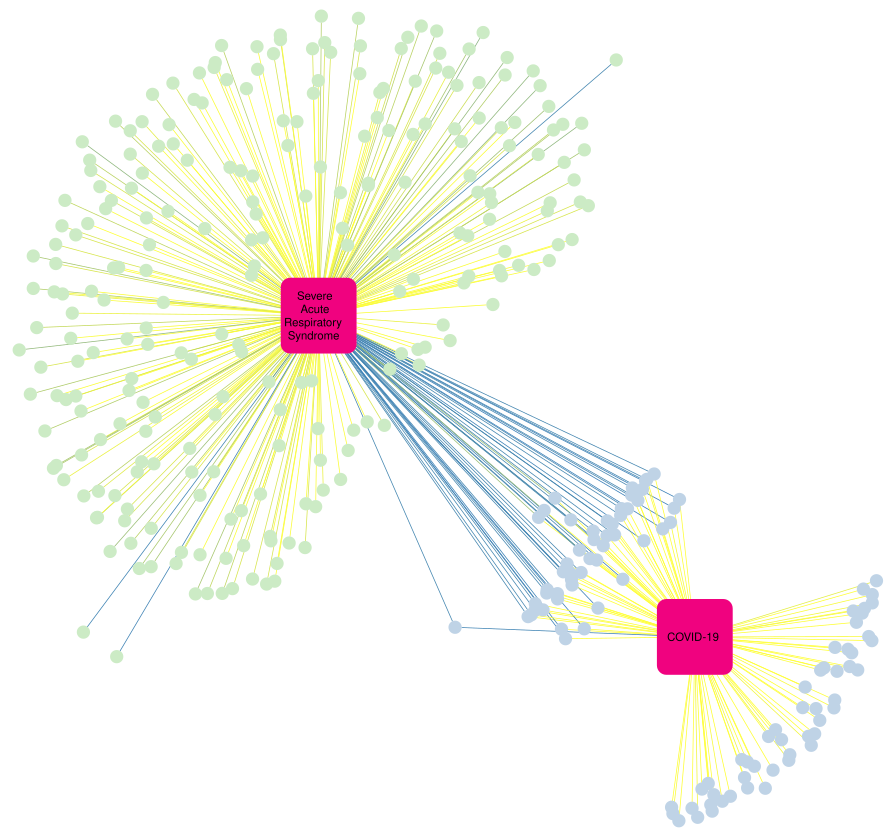
\includegraphics[width=\textwidth]{figures/COVID19xSARS_network.png}
        \caption{Network visualizing predicted repurposable drugs for COVID-19 and SARS. Yellow edges indicate a high adjusted similarity for the connected disease, while blue indicates a low value. Repurposable drugs associated with SARS are colored in green and drugs associated with COVID-19 are colored in blue.}
        \label{fig:Network}
    \end{subfigure}
     \hfill
     \begin{subfigure}[b]{0.45\textwidth}
         \centering
         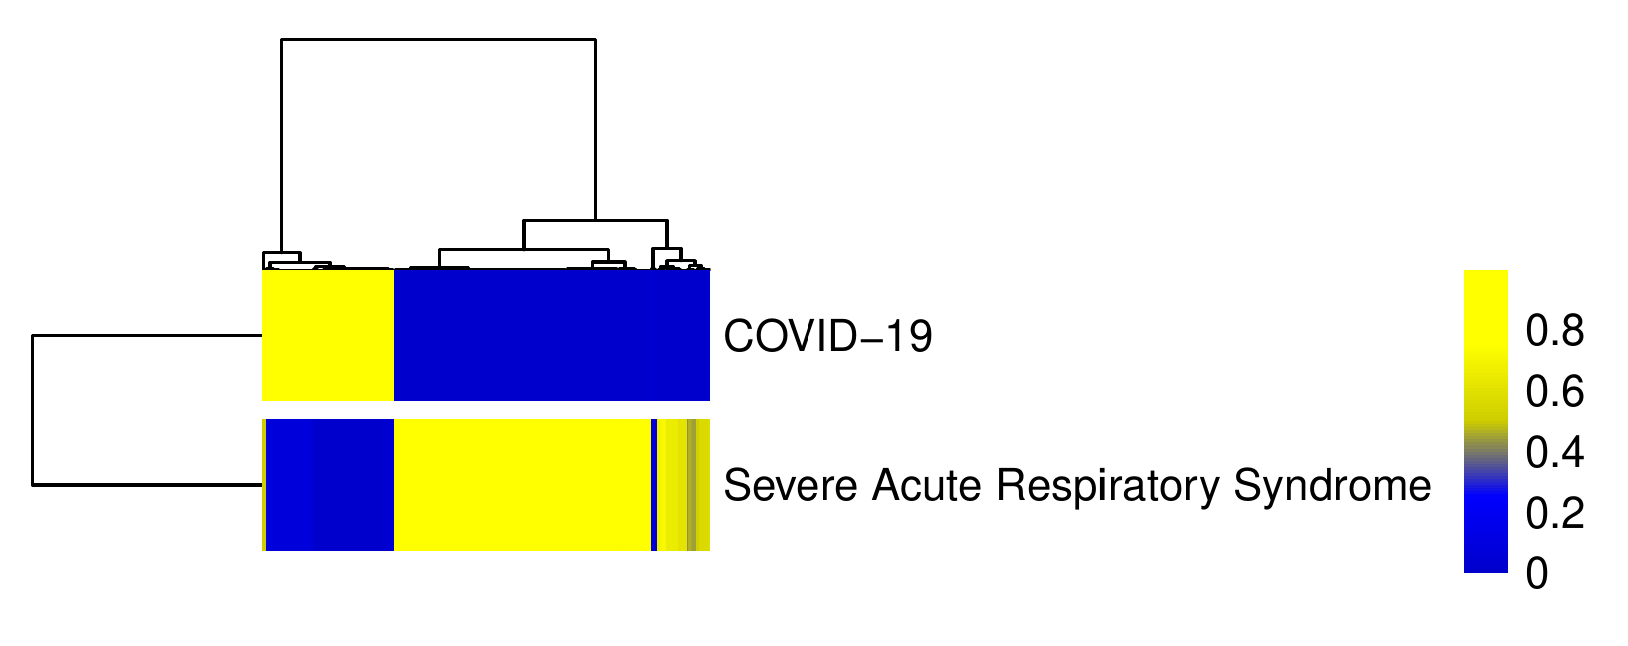
\includegraphics[width=\textwidth]{figures/Disease_Drug_Heatmap.png}
         \caption{Clusterd heatmap visualizing the adjusted similarity of both diseases per Drug. The color map ranges from blue (low) to yellow (high)}
         \label{fig:DrugDiesease}
     \end{subfigure}
     \hfill
     \begin{subfigure}[b]{0.45\textwidth}
         \centering
         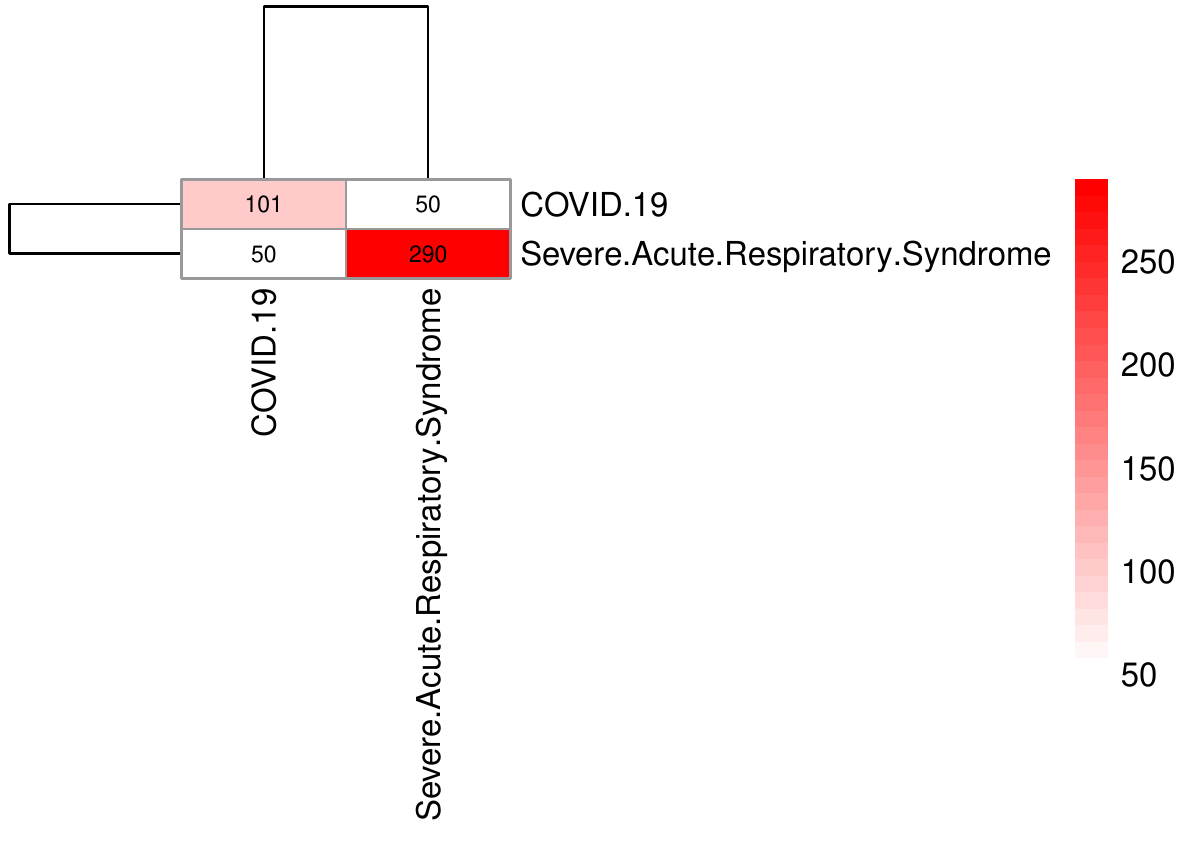
\includegraphics[width=\textwidth]{figures/Disease_Disease_Heatmap.png}
         \caption{clustered heatmap visualizing amount of shared  drugs between diseases.}
         \label{fig:DieseaseDiesease}
     \end{subfigure}
        \caption{Comparison of predicted repurposable drugs for COVID-19 and SARS.}
        \label{fig:SARS_COVID}
\end{figure}

The most notable drugs from this view are the ones that are shared and have high adjusted similarity for both diseases. The drugs for which this is the case are shown below. Table \ref{fig:predDrugsShared} shows the individual adjusted similarities per disease as well as the sum per drug.

\begin{table}[H]
\begin{center}

\captionsetup{width=9cm}
\caption{Predicted Drugs for both SARS and COVID-19 with the highest summed adjusted similarity for to both diseases. [\ref{sec:appendix}]}
\label{fig:predDrugsShared}

\npdecimalsign{.}
\nprounddigits{3}
\begin{tabular}{ l n{2}{5} n{2}{5} n{2}{5}}
    \toprule
    \text{Drug} & \text{COVID-19} & \text{SARS} & \text{Sum} \\
    \midrule
    \text{benazepril}  & 0.9932432669830258 & 0.504781792120694 & 1.4980250591037199  \\
    \text{cilazapril} & 0.9932432669830258 & 0.504781792120694 & 1.4980250591037199  \\
    \text{quinapril} & 0.9932432669830258 & 0.504781792120694 & 1.4980250591037199  \\
    \text{turoctocog alfa pegol} & 0.9932432669830258 & 0.161441849724981   & 1.1546851167080068 \\
    \bottomrule
\end{tabular}
\npnoround

\end{center}
\end{table}

The tabular data makes it clear that the drugs that have been predicted for both diseases are below non-shared drugs in similarity. However, the chance that these drugs might be repurposable for both diseases, makes the investigation worthwhile. 
All of the top 3 drugs shown in Table \ref{fig:predDrugsShared} share one interesting target \cite{Wishart2017}. This target is the aforementioned Angiotensin-converting enzyme (ACE). As stated above the ACE2 protein is required in order to allow the virus to enter the host cell. All three drugs act as inhibitors of ACE and are originally used for hypertension and heart failure \cite{Wishart2017}. Perhaps, this inhibition also prevents membrane fusion to be triggered by the virus.
The last drug of this subselection is Turoctocog alfa pegol. It is intended to be used to reduce the frequency and severity of bleeding episodes in Haemophilia patients \cite{Wishart2017}. Why this drug was predicted to be useful against COVID-19 and SARS requires further investigation.

% --------------------------------------------------------------------------------


%\clearpage

\section{Conclusions}

We could show that many potential candidates can act as repurposable drugs for the treatment of COIVD-19. Furthermore, it seems that the application of such a drug to also treat another known human coronavirus, Severe acute respiratory syndrome, seems non-trivial. This has interesting implications for the treatment of other coronavirus variants that may emerge in the future.
The candidate drugs discussed here represent only a fraction and analysis was solely based on pre-existing literature. It is important that all viable candidates are evaluated to undergo reduced clinical testing afterward. This process allows faster and more cost-effective development of new treatment strategies which is crucial to stay ahead of emerging and rapidly evolving diseases.

%----------------------------------------------------------------------------------------
%	Bibliography
%----------------------------------------------------------------------------------------
\clearpage

\printbibliography

%----------------------------------------------------------------------------------------
%	Appendix
%----------------------------------------------------------------------------------------
\clearpage
\section{Appendix}
\label{sec:appendix}

\subsection{Python scripts}

\subsubsection{Bar plot of onLabel diseases}

\begin{lstlisting}[language=python]
import pandas as pd

onLabel = pd.read_csv("./onLabel_COVID19_drug.txt", sep="\t")
tdd = onLabel["TTD_association"]
tdd.value_counts()
tdd = tdd.value_counts()
tdd_top = tdd[tdd > 1] # only include diseases with more than 1 occurrence
ax =  tdd_top.plot(kind="barh", ylabel="diseases occuring more than once")
fig = ax.get_figure()
fig.savefig('./onLabel_diseases_saverunner_covid.png')
\end{lstlisting}

\subsubsection{Finding common drugs between SARS and COVID-19}

\begin{lstlisting}[language=python]
import pandas as pd

df = pd.read_csv("./Drug_Disease_network_pval0.05.txt", sep="\t")
covid = df[df["disease"] == "COVID-19"]
sars = df[df["disease"] == "Severe Acute Respiratory Syndrome"]
common_drugs = pd.merge(
    covid[["drug", "adjusted_similarity"]],
    sars[["drug", "adjusted_similarity"]],
    how="inner",
    on="drug",
    suffixes=["_covid", "_sars"],
)
common_drugs.head()
common_drugs.sort_values(
    ["adjusted_similarity_covid", "adjusted_similarity_sars"], ascending=[False, False]
)
common_drugs["adj_sim_sum"] = (
    common_drugs["adjusted_similarity_covid"] + common_drugs["adjusted_similarity_sars"]
)
common_drugs.sort_values("adj_sim_sum", ascending=False)
common_drugs.to_csv("./common_drugs_sars_covid.csv")
\end{lstlisting}

\subsubsection{Sorting predicted drugs}

\begin{lstlisting}[language=python]
import pandas as pd

pd.options.display.float_format = "{:.5e}".format
df = pd.read_csv("./Drug_Disease_network.txt", sep="\t")
df = df.sort_values(["pval", "adjusted_similarity"], ascending=[True, False])
df.to_csv("./COVID19_drugs_sorted_pval_adjsim.csv", float_format='%.3e')
\end{lstlisting}



\end{document}
